%
% file : Rapport.tex
% date : dec 2017
% author : Jean-Marie Saindon <jsaindon@enseirb-matmeca.fr>, Achram ElKhamsi <aelkhamsi@enseirb-matmeca.fr>
% brief : Projets5 groupe 3723 Rapport
%

\documentclass[a4paper]{article}

\usepackage[utf8]{inputenc}
\usepackage[french]{babel}
\usepackage{graphicx}
\usepackage{lmodern}
\usepackage{multicol}
\usepackage{fancybox}
\graphicspath{{./img/}}
\usepackage{amsmath, amsfonts, amssymb}
\usepackage[left=3cm,right=3cm,top=2cm,bottom=2cm]{geometry}
\usepackage{url}
\usepackage{color}
\usepackage{lmodern}
\usepackage{amsmath}
\usepackage{amssymb}
\addto\captionsfrench{\renewcommand{\chaptername}{Partie}}
\addto\captionsfrench{\def\figurename{Image}}
\addto\captionsfrench{\def\tablename{Tableau}}
\addto\captionsfrench{\renewcommand{\listfigurename}{Table des images}}
\addto\captionsfrench{\renewcommand{\bibname}{R\'ef\'erences}}
\renewcommand\appendixname{Annexes}

\begin{document}
\begin{titlepage}
\begin{center}


\includegraphics[width=0.6\textwidth]{logo_enseirb}\\[1cm]

{\large Fillière Informatique 1ère année}\\[0.5cm]

{\large Groupe 3723}\\[0.5cm]

% Title
\rule{\linewidth}{0.5mm} \\[0.4cm]
{ \huge \bfseries Rapport Projet Semestre 5: \\[0.4cm]
				Kitty Wonderland : A Battle of wits \\[0.4cm]}
\rule{\linewidth}{0.5mm} \\[1.5cm]

% Author and supervisor
\noindent
\begin{minipage}{0.4\textwidth}
  \begin{flushleft} \large
    \emph{Auteurs :}\\
    M. Jean-Marie \textsc{Saindon}\\
    M. Achraf \textsc{El Khamsi}
  \end{flushleft}
\end{minipage}
\begin{minipage}{0.4\textwidth}
  \begin{flushright} \large
    \emph{Encadrants :} \\
    Pr. Pierre \textsc{Huchant}\\
    Pr. Laurent \textsc{Chancogne}
  \end{flushright}
\end{minipage}

\vfill

% Bottom of the page
{\large Version du\\ \today}

\end{center}
\end{titlepage}
\newpage
\tableofcontents
\newpage
% introduction
% - présenter le sujet,
% - définir le cadre de travail,

\section{Introduction}
\subsection{Présentation du sujet}

Dans le cadre de la réalisation de ce projet, l'objectif était de mettre en place la simulation d'un jeu de cartes dans lequel 2 joueurs ou plus s'affrontent sur un plateau de jeu.\\

Les joueurs possèdent plusieurs caractéristiques parmis lesquelles on retrouve les points de vie, les points de mana (permettant au joueur d'utiliser des cartes), le gain (s'additionnant au points de mana au début de chaque tour) ainsi que l'ensemble des cartes qui composent la du joueur (Les cartes ayant un cout en mana et un effet sur le joueur la possèdant ou sur l'un de ses adversaires). La probabilité qu'un joueur pioche une certaine carte est inversement proportionelle à son coût.L'issue de la partie peut se concrétiser par le sacrement d'un vainqueur ou par un match nul.

\subsection{Définition du cadre de travail}

La réalisation de ce projet s'est effectuée en binôme, en langage C et avec l'aide du logiciel de version subversion. La progression du projet à suivi une logique d'achievement. Cela consiste premièrement en la réalisation de la mécanique du jeu (Baseline) puis en l'ajout d'extensions (les achievements) à celle-ci afin de l'améliorer.\\

La mise en place de la Baseline ainsi que l'aclimatation à l'environnement de travail s'est entièrement faite à deux sur un même ordinateur. Cette étape nous a permis de découvrir le projet ensemble et d'en discuter afin d'adopter la même vision de ce qu'il devait devenir. Par la suite, la meilleure compréhension des objectifs à atteindre et l'entente nous a permis de travailler en parallèle et ainsi de gagner en efficacité sur les achievements qui ont suivis.\\

Pour chaque achievement, nous avons adopter la procédure suivante: Premièrement, la lecture des directives de l'achievement, puis une discution pour décider de la manière adéquate pour la réalisation de celles-ci. Ensuite venait l'étape de l'implémetation dans laquelle des réajustements pouvaient intervenir. Finalement, le codage s'achevait par une phase de tests.
\newpage
% parties pour chaque achievement
% - analyser les problèmes rencontrés,
% - détailler la conception des solutions algorithmiques,
% - discuter de la correction et de la complexité des algorithmes,
% - évaluer des problèmes de mise en oeuvre et de la réalisation,
% - et décrire les tests de validation.

\section{Etapes du projet}
\subsection{Baseline}
\subsubsection{Directives}

L'objectif de cette partie est d'établir une définition des types joueur, carte et plateau de jeu ainsi que de coder la dynamique du jeu (Phase de jeu). De plus, il faudrait implémenter des fonctions d'affichages permettant de connaitre l'état de chaque joueur à chaque tour (Phase d'affichage).
Chaque phase abritera différentes sous-phase que nous allons expliciter par la suite.

L'architecture de notre programme principale suit le modèle suivant :
\begin{center}
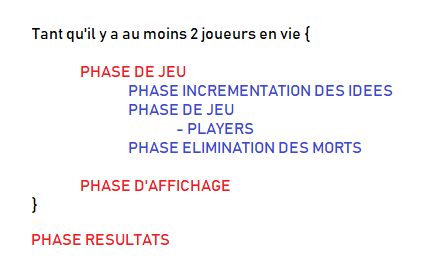
\includegraphics[width=0.6\textwidth]{Baseline}\\[1cm]
\end{center}
\subsubsection{Choix de modélisation}

Trois types abstrait sont indispendable pour la première version du jeu, à savoir la structure player (joueur), card (carte) et board (plateau de jeu).\\
\begin{center}
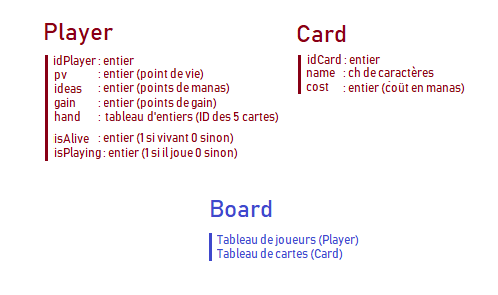
\includegraphics[width=0.6\textwidth]{Baseline_1}\\[1cm]
\end{center}
\noindent
\begin{itemize}


\item \textbf{Card} :
Le type abstrait card représente une carte. Chaque carte a un ID qui facilitera sa manipulation, un nom et un coût

\item \textbf{Player}: 
Le type abstrait player représente un joueur. Chaque joueur a un ID qui facilite sa manipulation et le différencie d'un autre, ainsi que des points de vie, d'idées et de gain. La main du joueur est représenté par un tableau d'entiers qui contient les ID des cartes du joueur, (un tableaux d'entiers est plus simple à manipuler qu'un tableau de carte) le champ isAlive (resp isPlaying) vaut 1 si le joueur est vivant (resp si c'est son tour de jouer), 0 sinon.

\item \textbf{Board} :
La structure de plateau de jeu a pour principal fonction de rassembler toutes les variables abstraites dans des tableaux. 

\end{itemize}

\subsubsection{Solutions algorithmiques}

On va présenter çi-dessous les principales fonctions de la Baseline. Ces fonctions abritent plusieurs sous-fonctions qu'on va pas citer 


\begin{enumerate}

\item \textbf{La phase de jeu} \\
\begin{itemize}  

\item increase\_ideas : Ajoute la valeur du gain d'un joueur à ses points d'idées (Phase d'incrémentation des idées )\\
\item select\_card : Choisit une carte aléatoirement depuis la main du joueur \\
\item apply\_card  : Applique l'effet de la carte choisit précédement par la fonction select\_card \\
\item refill\_cards  : Si le joueur a joué une carte, cette fonction pioche une carte selon un processus probabiliste (Chaque carte a une probabilité d'être pioché inversement proportionnele a son coût)\\
\item kill\_players  : Elimine les joueurs qui ont un point de vie nul ou négatif \\
\end{itemize}
\item \textbf{La phase d'affichage} \\

\begin{itemize}
\item display\_players  : Affiche chaque joueur vivant ainsi que ses points de vie, d'idées et de gain, puis affiche les noms des cartes dont il dispose \\
\begin{center}
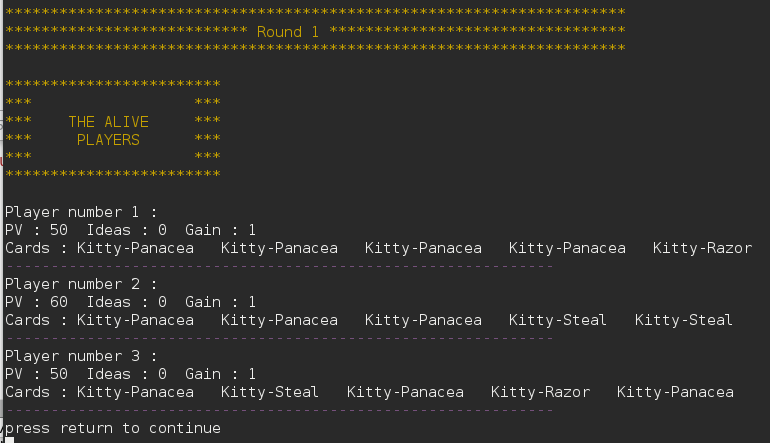
\includegraphics[width=0.6\textwidth]{display_players}\\[1cm]
\end{center}
\end{itemize}
\item \textbf{La phase des résultats} \\
\begin{itemize}
\item announce\_results : Le seul joueur vivant est déclaré gagnant \\
\begin{center}
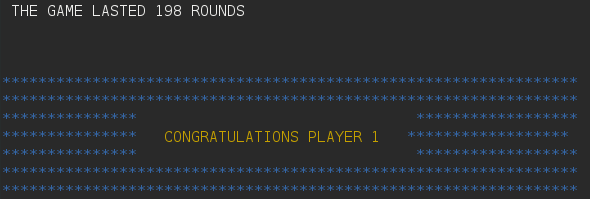
\includegraphics[width=0.6\textwidth]{anounce_results}\\[1cm]
\end{center}
\end{itemize}

\end{enumerate}

\subsubsection{Complexité des algorithmes}

Les fonctions select\_player, display\_players, kill\_players ont des complexités en temps linéaires relativement au nombre de joueurs car la plupart de celles-ci parcourent le tableau des joueurs disponible dans le plateau de jeu\\

Pour toutes les autres fonctions ont retrouve une complexité en temps (et en espace) constante
\newpage
\subsection{Achievement 1}
\subsubsection{Directives}

L'objectif de cet achievement est de remplacer le tirage aléatoire des cartes à chaque pioche par un tirage dans un memento (deck) propre à chacun des joueurs et constitué en début de partie. Ce deck sera implémenté par une structure de file, une pioche correspondant a un defile et une défausse correspondant a un enfile. Après avoir effectué 50 pioches dans le deck on doit le mélanger. 

\subsubsection{Choix de modélisation}

Un type abstrait file a été implémenté pour satisfaire cet achievement. Le type abstrait player a également été enrichi.\\ 
\begin{center}
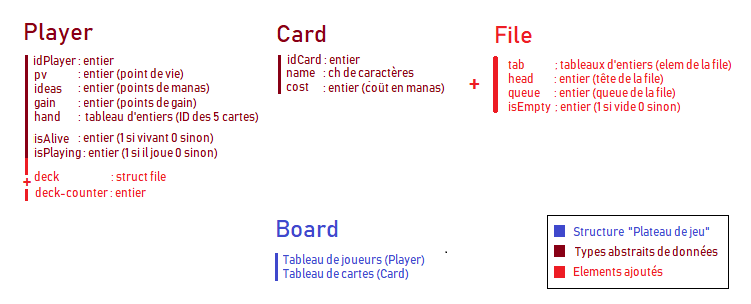
\includegraphics[width=0.6\textwidth]{Ach1}\\[1cm]
\end{center}

\begin{itemize}

\item \textbf{File}: 
La structure de file que nous avons décidé d'implémenter a été munis des champs suivants : head (indice de tête de la file), queue (indice de fin de la file), tab (tableau dans lequel on stocke les éléments de la file) et isEmpty (indiquant si la file est vide). Ce dernier est nécessaire pour faire la différence entre une file vide et une file pleine car dans les deux cas les indices de tête et de queue sont identiques.\\

\item \textbf{Player}: 
Le type abstrait player a été enrichi d'un champ deck (étant une structure file). Nous avons de plus ajouté un champ deck\_counter a cette même structure pour pouvoir connaitre le nombre de pioches effectuées (et ainsi appelé une fonction de mélange après 50 pioches)\\
\end{itemize}

\subsubsection{Solutions algorithmiques}
On va présenter çi-dessous les principales fonctions répondant aux éxigences de cette version du jeu\\
\begin{itemize}  

\item length\_file : Cette fonction retourne la taille d'une file (entre le curseur head et le curseur queue) \\
\item fill\_deck  : Cette fonction rempli une file avec l'ID des Cartes selon les probabilités de tirages demandées\\
\item defile : Cette fonction retire l'élément en tête de la file \\
\item enfile  : Cette fonction ajoute l'élément en queue de file \\
\item mix\_file  : Le principe de mélange appliqué a un tableau f'entiers est le suivant : On parcourt le tableau de l'indice 0 à n-2. Lors de notre parcours, le i iem élèment du tableau sera échanger aléatoirement avec l'un des élèments d'indice compris entre i+1 et n-1. Cette fonction applique le même principe à notre file\\\\
\end{itemize}

La fonction defile est équivalente à piocher une carte . Quand une carte est jouée, elle est insérée dans la file ( enfile ), et quand toutes les cartes de la file sont jouées (aprés 50 pioches), la file est mélangée ( mix\_file )


\subsubsection{Complexité des algorithmes}

Les fonctions implémentées dans cette version du jeu ont une complexité en temps constante. length\_file, mix\_file et fill\_deck ont une complexité linéaire en fonction de la taille de la file fournie, si on considére celle-çi variable, sinon la compléxité est constante. Quant à la compléxité en espace, elle est toujours constante, car les fonctions utilise des files qui ont déja était définis auparavant.

\newpage
\subsection{Achievement 2}
\subsubsection{Directives}
La deuxième version du jeu consiste à doter le jeu d’une dimension spatiale. Les joueurs peuvent désormais occuper une place au sein d’une une grille 50x50 et se déplacer à chaque tour. Cependant, des cases peuvent aussi être occupés par un bloc de caramel, dans ce cas ils sont infranchissables par les joueurs.

Une nouvelle phase sera ajoutée à notre programme: la phase de mouvement
\begin{center}
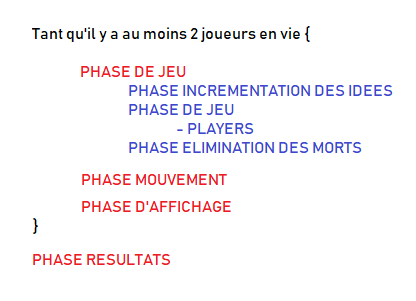
\includegraphics[width=0.6\textwidth]{Ach2_1}\\[1cm]
\end{center}

\subsubsection{Choix de modélisation}
Afin de réaliser cette version du jeu, une modification des structures existantes ainsi qu’une implémentation de nouvelles structures sont nécessaires : \\

\begin{center}
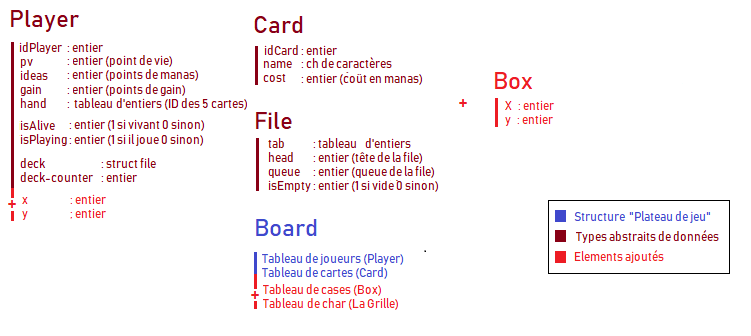
\includegraphics[width=0.6\textwidth]{Ach2}\\[1cm]
\end{center}

\begin{itemize}
\item Structure \textbf{box}  :   création d’une structure représentant une case de la grille, qui a comme champs ses coordonnées x et y \\
\item Structure \textbf{board}  :
\begin{itemize}
\item Ajouter un tableau de caractère de dimension double comme nouveau champ de notre structure, de taille 50x50 et qui représentera notre grille 
\item Ajouter un tableau de box (de longueur le nombre de joueurs) aux champs de notre structure, il va nous être utile au niveau des conflits de déplacement entre joueurs.\\
\end{itemize} 

\item Structure \textbf{player}  :  Ajouter deux entiers (x et y) comme nouveaux champs de notre structure, ils représenteront les coordonnées d’un joueur dans la grille.
\end{itemize}

\newpage
\subsubsection{Solutions algorithmiques} 

\begin{enumerate}
\item \textbf{Initialisation de la grille} \\
\begin{itemize}
\item Initialize\_arena : on a besoin en début de partie de positionner les joueurs dans la grille. Cette fonction se charge de choisir aléatoirement à chaque joueur deux coordonnées et de placer son ID dans la case correspondante. Elle évite éventuellement que deux joueurs aient les mêmes coordonnées.\\
\end{itemize} 
\item \textbf{Phase mouvement} \\
\begin{itemize}
\item Choose\_directions: en fonction de la position de chaque joueur, cette fonction choisit aléatoirement une case vide parmi les quatre cases qui l’entourent, et stocke la case dans le tableau de cases (disponible dans le board) à l’indice correspondant à l’ID du joueur. \\
\item Del\_duplicates : cette fonction parcourt le tableau de cases, qui représente désormais les cases qui vont être visitée par chaque joueur, et met les cases semblables à (-1, -1). Cela va permettre de résoudre les conflits entre les joueurs souhaitant se déplacés vers la même case \\
\item Move\_all : Cette fonction affecte chaque joueur à la case correspondante à son ID dans le tableau de cases (box). Si la case est à (-1, -1), le joueur ne bouge pas. (Cette fonction englobe les deux dernières)\\
\end{itemize}

\item \textbf{Nouvelles Cartes}\\
\begin{itemize}
\item Kitty\_Stone : Cette carte choisit un adversaire ainsi qu’une case vide l’entourant, en suivant un processus aléatoire, et affecte à cette case un bloc infranchissable représenté par '\textcolor{red}{\#}'\\

\end{itemize}

\item \textbf{Affichage de la grille}\\
\begin{itemize}
\item Display\_arena: Cette fonction parcourt la grille et affiche le contenu de chaque case, ‘0’ pour une case vide, l’ID du joueur en \textcolor{green}{vert} s’il est vivant, en \textcolor{red}{rouge} sinon, et ‘\textcolor{red}{\#}’ si c’est un bloc infranchissable\\

\begin{center}
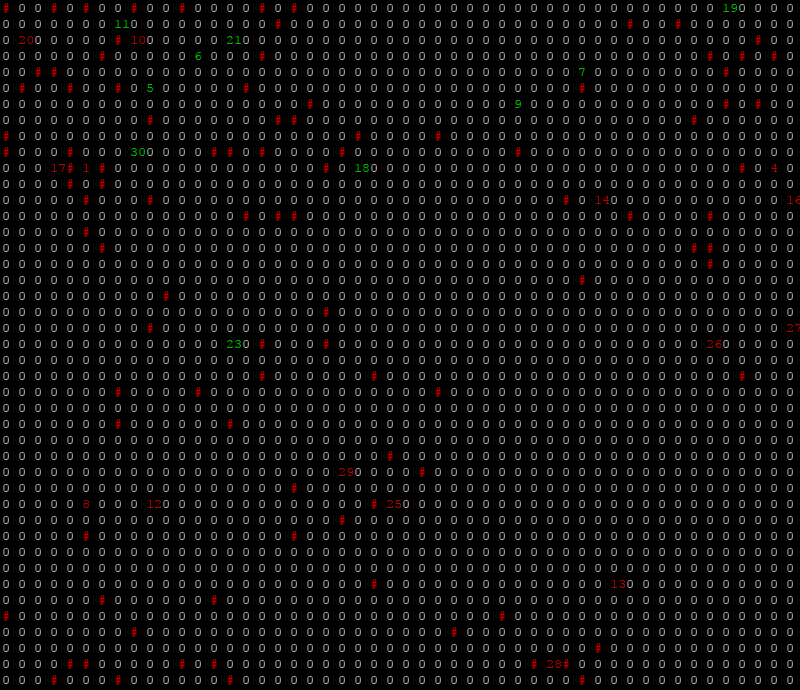
\includegraphics[width=0.6\textwidth]{arena}\\[1cm]
\end{center}
\end{itemize}

\end{enumerate}

\newpage
\subsubsection{Complexité des algorithmes}
Les fonctions implémenté dans cette version du jeu ont quasiment toutes une compléxité en temps linéaire et en espace constante, parce qu'on parcourt fréquemment des tableaux de taille égale au nombre de joueurs (qui peut varier) \\

La fonction display\_arena peut paraître avoir une compléxité en temps quadratique, Ce serait la cas si la taille de la grille peut varier, alors que dans notre implementation on a considérés que sa taille était fixe (50x50) 

\newpage
\subsection{Achievement 3}
\subsubsection{Directives}
Dans un but d’enrichir la dynamique du jeu, la troisième version de Kitty Wonderland permettra désormais aux joueurs d’invoquer des amis sur le plateau de jeu. Ces derniers auront une seule carte et une seule cible qu'peuvent attaquer quand ils ont assez de points de d'idées, cependant ils ne peuvent joueur qu’un maximum de 20 tours avant de disparaître.\\

Cette modification affectera la Phase de jeu de notre programme, une section dédiée aux amis des joueurs sera ajoutée:

\begin{center}
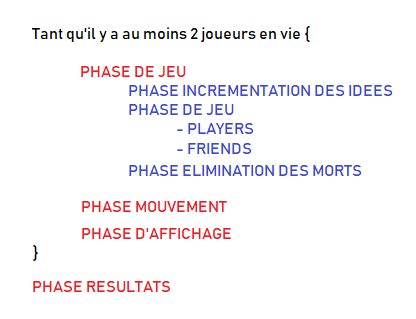
\includegraphics[width=0.6\textwidth]{Ach3_3}\\[1cm]
\end{center}

\subsubsection{Choix de modélisation}
Afin de réaliser cette version du jeu, on a pensé à utiliser une structure en liste chainée car on ne sait pas préalablement le nombre d’ami que peut avoir un joueur.\\

Un ami aura le même ID que le player (ou le friend) qui l’a joué, comme ça on distinguera les différentes «équipes» évoluant dans le jeu, chacune formé par un joueur et ses amis. L’ID joue le rôle d’un nom de famille.\\

\begin{center}
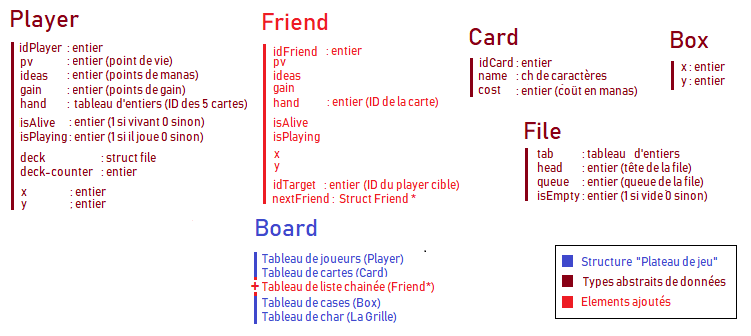
\includegraphics[width=0.6\textwidth]{Ach3}\\[1cm]
\end{center}

\begin{itemize}
\item Structure \textbf{Friend}:   Cette structure représentera un nœud de la liste chainée lié à chaque joueur. Ce nœud à comme valeurs (approximativement) les mêmes champs que la structure Player, et dispose d’un pointeur vers le prochain ami appartenant à la même équipe\\
\item Structure \textbf{Board}: Nous allons ajouter aux champs de cette structure un tableau de liste chainée. L’indice d’une liste chainée dans le tableau correspond à l’ID du joueur «père»\\
\end{itemize}

\newpage
\subsubsection{Solutions algorithmiques}
\begin{enumerate}
\item \textbf{Creation d’un ami}
\begin{itemize}
\item Choose\_coord: Cette fonction choisit aléatoirement une case vide parmi celles qui entourent le joueur (ou l’ami) qui a invoqué l’ami, s’il n’y a aucune case vide, la fonction renvoie la case (-1, -1)\\
\item Select\_target: Cette fonction choisit aléatoirement une cible n’ayant pas le même ID que le joueur (ou l’ami) qui à invoqué l’ami\\
\item Kitty\_Puppy: Cette carte crée un ami, initialise ses champs, ses coordonnées (choose\_coord) et sa cible (select\_target), puis l’insère dans la liste chainée correspondante à son ID. Si la fonction choose\_coord renvoie la case (-1, -1), l’ami n’est pas créé parce qu'il n'a pas où apparaître.\\
\end{itemize}

\item \textbf{Phase de jeu}\\\\
La phase de jeu relatifs aux Friends suivra le modèle suivant :
\begin{center}
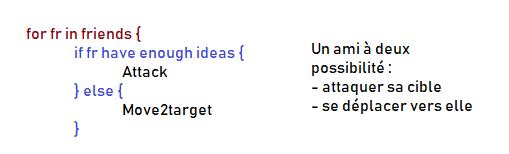
\includegraphics[width=0.6\textwidth]{Ach3_1}\\[1cm]
\end{center}
\begin{itemize}
\item Attack: Cette est équivalente à la fonction apply\_card pour les joueurs. Dans ce cas, elle applique l’effet de l’unique carte du joueur sur sa cible\\
\item Move2target: Cette fonction permet à un ami de s’approcher de sa cible, elle calcule la distance entre la coordonnée x du joueur et celle de la cible de deux façons et décide de l’évolution de la coordonnée x de l’ami en fonction de la plus courte distance (même chose pour la coordonnée y) :
\begin{itemize}
\item Distance directe:  val.abs( xFriend – xTarget ) 	
\item Distance prenant en compte la nature torique de la grille: 48 -val.abs( xFriend - xTarget)

\begin{center}
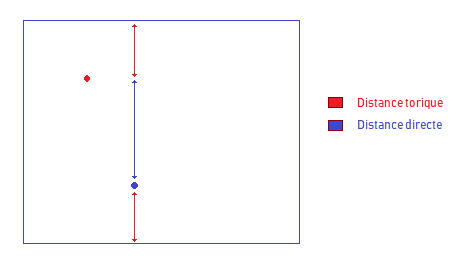
\includegraphics[width=0.6\textwidth]{Ach3_2}\\[1cm]
\end{center}
\end{itemize}
\item Kill\_friends : élimine les amis qui n’ont plus de PV, dépassant 20 tours de jeu ou ceux dont le joueur portant le même ID est mort.\\
\item Reselect\_target : Parcourt les amis de chaque joueur, si la cible d’un ami est morte, cette fonction lui affecte une nouvelle cible\\

\end{itemize}
\newpage
\item \textbf{Autres modifications}\\

Les cartes de jeu auront de nouvelles versions qui permettront leur utilisation par un Friend contre un Player et vice versa, ce qui entrainera la modification de la fonction apply\_card


\end{enumerate}


\subsubsection{Complexité des algorithmes}

Toutes les fonctions ont une complexité en espace constante. les fonctions Attack et Move2target ont une compléxité en temps constante alors que Kill\_friends et Reselect\_target ont une complexité en temps linéaire relativement au nombre de joueur,  elle peut au pire des cas tendre vers une complexité quadratique en prenant en considération le nombre d'amis de chaque joueurs

\newpage
\subsection{Tests de validation}


Le protocole suivi dans la quasi-totalité des tests était de créer une variable plateau de jeu puis d'initialiser tout ses champs, ce qui initialisera par conséquence les joueurs, les cartes et la grille. Ensuite les tests ont étè implémenter de façon à s'assurer du bon fontionnement d'un cas usuelle, puis des cas limites. Ces tests ce sont avérés utiles puisqu'ils nous ont permis de remonter rapidement aux différentes erreurs et disfonctionnement de notre programme 

Les tests de l'achievement 3 sont séparé des autres tests parce que les codes sources de cette version du jeu ont été modifiés, ce qui ne permettrait pas de faire fonctionner correctement les tests des versions précédentes\\\\\\\\

\section{Conclusion}

A travers ce projet, notre niveau en terme de programmation et de manipulation de structure est nettement amélioré. On a eu l'occasion d'approfondir notre connaisance au niveau de la compilation séparée, de la manipulation des types abstraits de données et surtout au niveau de l'organisation du code source.

la confrontation aux multiples erreurs et disfonctionnement nous a appris qu'un bon contrôle du code source est essentiel dans tout projet, et a enrichi notre connaisance sur le fonctionnement de l'ordinateur au point que les problèmes étaient résolu plus rapidement et plus efficacement qu'avant.

\end{document}
